%%%%%%%%%%%%%%%%%%%% author.tex %%%%%%%%%%%%%%%%%%%%%%%%%%%%%%%%%%%
%
% sample root file for your "contribution" to a proceedings volume
%
% Use this file as a template for your own input.
%
%%%%%%%%%%%%%%%% Springer %%%%%%%%%%%%%%%%%%%%%%%%%%%%%%%%%%


\documentclass{svproc}
%
% RECOMMENDED %%%%%%%%%%%%%%%%%%%%%%%%%%%%%%%%%%%%%%%%%%%%%%%%%%%
%

% to typeset URLs, URIs, and DOIs
\usepackage{url}
\usepackage{float}
\usepackage{graphicx}
\def\UrlFont{\rmfamily}

\def\UrlBreaks{\do\/\do-}
\usepackage{breakurl}

\begin{document}
\mainmatter              % start of a contribution
%
\title{A Deep Learning approach for detecting medical face mask on human faces in response to Covid19}
%
\titlerunning{Medical Face Mask Detection}  % abbreviated title (for running head)
%                                     also used for the TOC unless
%                                     \toctitle is used
%
\author{Borun Das\inst{1} \and Mahmud Hasan\inst{2} \and Rafi Belal \inst{3}}
%
\authorrunning{Borun Das et al.} % abbreviated author list (for running head)
%
%%%% list of authors for the TOC (use if author list has to be modified)
\tocauthor{Borun Das, Mahmud Hasan}
%
\institute{Learning Imaging Lab, Bangladesh\\
\email{nilborun@gmail.com},
\and
University of Western Ontario, Canada\\
\email{mhasan62@uwo.ca},
\and
Center for Analysis, Research and Development, Bangladesh \\
\email{rafi2213@yahoo.com}}
\maketitle              % typeset the title of the contribution

\begin{abstract}
In this difficult time of COVID19, using a facial mask is a life saver, specially in all indoor public places. In this work, a deep learning based approach is proposed that detects whether or not a human face contains a face mask. The proposed method is capable of detecting the facial mask with $98\%$ accuracy for any frontal face static image or videos. The validation was performed on a variety of different scenarios to ensure the accuracy.
% We would like to encourage you to list your keywords within
% the abstract section using the \keywords{...} command.
\keywords{deep learning, face mask detection, Covid19}
\end{abstract}
%
\section{Background}
%
COVID19 pandemic hit the world hard in the year 2020, both economically and medically. On one side, we discovered that human beings are so vulnerable against mother nature even after having so many advancement in science and technology. On the other side, we also found ourselves in extreme financial difficulties as businesses around the world has been suffering due to lack of customers and demands. Although a few vaccine candidates were developed, tested and started mass vaccination towards the end of the year, scientists are yet to confirm the overall efficiency, side effects, time the created antobodies are effective for and so on. Even if the vaccines work perfectly, it will take years to develop billions of doses and vaccinate people around the world. And until that, personal protective equipment (PPE) that the front line workers and people have been using is our lifeguard. World Health Organization (WHO) advised that among all of the PPEs available, face masks are the most protective as they directly cover nose and mouth - two most susceptible areas of human body. Another vulnerable area is the eyes, and WHO also suggested to use safety goggles, specially for the health service workers. For general people, however, the face mask at the minimum. \\

\par Now although people around the world are advised to use face mask in all indoor places and recommended in outdoor, it was not very uncommon to see that many people are ignoring the face mask or not properly using them, putting all of us at risk. We have also seen movement against using face masks that forced many countries/authorities to enforce the usage of face masks in indoor public spaces. Authorities/officials were also seen using thermal detector to detect people's temperature before letting them enter any public space. While using a thermal gate at the entry point was easy to make this work (semi) automated, checking whether or not every person was using face mask was not that easy, due to unavailability of related technology. The automated technologies that authorities have been using around the world are mostly about detecting face, not face masks. So, this had to be done mostly manually, and enforcement became difficult causing more and more positive cases over the time almost everywhere. \\

In this work, we came up with a deep learning based approach to automatically detect whether or not a person is using face mask from both static and video images. The outcome can be used behind any camera currently in effect to detect if the person entering a space is using the face mask. It is similar to the thermal gate installed to detect the temperature and notify the authority if temperature is above a certain threshold for an subject (human). In similar manner, our proposed work is able to detect and notify the authority if the subject is not wearing the face mask properly, making the enforcement and warning easier. The proposed method was properly tested to verify that for any frontal face image/video, it is able to detect \emph{mask/no mask} correctly. The performance analysis showed that for any situation (out of 9 different testings performed) the proposed method is able to achieve $98\%$ accuracy.   

\section{Related Works}

Detection of facial mask is a comparatively new area of work. Before this pandemic started, there was almost no need to pay attention to this area. As a result, although we get thousands of works related to face detection or facial expression detection, we don't get much works related to face mask detection. In 2017, Ge et al. \cite{ge2017detecting} first worked on in this area.  In 2020, there have been a few publications indicating that people started focusing on this problem. \\

\par Loey et al. \cite{loey2020fighting} proposed a novel deep learning model based on YOLO-v2 and ResNet-50 for detecting medical masks from human face. They used two publicly available data set called \emph{MMD} and \emph{FMD} in their work. They were able to achieve $81\%$ accuracy as compared to Ge at el. who achieved around $76\%$ of accuracy. Loey et al. also proposed another hybrid model \cite{loey2020hybrid} where they used three different data sets such as Real World Masked Face Data set (RMFD), Simulated Masked Face Data set (SMFD) and Labeled Faces in the Wild (LFW). While for the first two data sets they were able to achieve only around $94\%$ and $96\%$ respectively, for the third data set they were able to achieve $98\%$ accuracy. \\

\begin{figure}[!ht]
\includegraphics[width=0.9\textwidth]{flowChart.png}
\centering
\caption{Flow chart of the proposed system.}
\label{flowChart}
\end{figure}

\par Mohan at el. lately proposed another tiny DeepNet model for facial mask detection for resource constrained endpoints \cite{mohan2020tiny}. They used the Kaggle data set and reported a $99.81\%$ accuracy in their proposed model. However, it's worth noting that the Kaggle data set has only $440$ images that contains equal number of mask and non-mask images. Chen at el. proposed a transfer learning technique to classify the mask/non-mask images, however they did it on a semi-synthetic data set.Trying on AlexNet and VGG16, they reported a validation accuracy of $ 96\%$ and $99\%$, respectively \cite{chen2020efficient}. The last reference that we found related is by Chowdary at el. \cite{chowdary2020face}. They only used SMFD data set mentioned above and reported $100\%$ accuracy. \\

\par Given all the  related works we found that there is no work that combine all the available data sets together and observe the responses, most of the works are focused on one or two data sets. So the accuracy reported by them are limited. Also, only one of the papers reported their training time, so finding a faster learning model is yet to be achieved. No previous work was found so far that also tested their method on video, therefore building a system that equally works for both video and still pictures is in scope, opening up the real application of the system behind the CCTV/Security Camera is a large indoor public space. 

\section{Proposed Method}

The model we are proposing is outlined in table \ref{modelTable}. Our proposed method is simple and straight forward. As the model shows, we used a combination of CNN with Max Pooling cascaded one after another, with the input size being reduced in next set. We then flatten the output data followed by a dense operation in order to pass the extracted feature to the Neural Network. This classifier is a binary classifier, it learns to classify a facial image either as with mask or without mask scenario. Fig. \ref{flowChart} shows the work flow of the proposed system. Before training the model, we re-scaled the images based on different parameters. Beside that, we provided validation images to the model during training so that we can calculate the validation accuracy before acquiring test accuracy and compare both. The accuracy we found on test data required only $6$ epochs while some of related works mentioned earlier had more than 100 epochs. So in terms of training time, our model is the fastest.

\begin{table}[!ht]
\centering
\begin{tabular}{llll}
\hline
Layer (type) &  Output Shape & &  Param \\
\hline
Conv2D & None, 148, 148, 32 & & 896 \\
MaxPooling2D & None, 74, 74, 32 & & 0 \\
Conv2D & None, 72, 72, 32 && 9248 \\
MaxPooling2D & None, 36, 36, 32 & & 0 \\
Conv2D) & None, 34, 34, 64 & & 18496 \\
MaxPooling2D & None, 17, 17, 64 & & 0 \\
Flatten & None, 18496 & & 0 \\
Dense & None, 64 & & 1183808 \\
Activation & None, 64 & & 0 \\
Dropout & None, 64 & &  0 \\ 
Dense & None, 1 & &  65 \\
Activation & None, 1 & &  0 \\
\hline \\
Total params: 1,212,513 \\
Trainable params: 1,212,513 \\
Non-trainable params: 0 \\
\hline \\
\end{tabular}
\caption{The description of the proposed model}
\label{modelTable}
\end{table}

\section{Results}

\subsection{Data Sets}
We have used the following datasets publicly available as cited in this work. Each data set has a different number of mask/no-mask combinations, giving us a total of $20,124$ mask and $12,748$ no-mask images.
\begin{enumerate}
  \item Face Mask Detection Data Set by Kaggle \cite{kagglefacemask}. 
  \item Simulated Masked Face Dataset (SMFD) \cite{smfd}.
  \item Real-World Masked Face Dataset (RMFD) \cite{wang2020masked}.
  \item Face-Mask-Detection Data set \cite{chandrikadeb7}.
  \item Real and Fake Face Detection Dataset \cite{realAndFakeFace}.
  \item MaskedFace-Net \cite{learned2016labeled}.
\end{enumerate}

\subsection{Experimental Setup}

We have designed our training and testing strategies as follows. We divided our data into two parts: real face-mask and simulated face-mask images. In both parts we have masked and non-masked images. Now during training and testing we further divided our images into two more parts: training and testing with specifying the Region of Interest (ROI/Face) and without specifying so. So finally the training and testing combinations are $(i)$ real face images with/without ROI and $(ii)$ simulated face images with/without ROI. We have another $(iii)$ category called real images with multiple persons present or full body present (i.e. not only face) and we have the two sub-categories of with/without ROI there as well. Now we mixed both real and simulated image set together as $(iv)$ and subdivided it similarly with and without specifying ROI. These combinations give us a total of 8 different training testing scenario. Finally we make a combination of everything and trained and tested the model. A summary of all the experimental results is given in Table \ref{expResult}. The test accuracy reported in Table \ref{expResult} was obtained by the \emph{evalute} function of tensorflow/keras.

\begin{table}[]
\centering
\begin{tabular}{lc}
\hline
Data & Test Accuracy \\
\hline
Real face with full body/multiple persons present & 0.99 \\
Real face with ROI detected only                       & 0.98 \\
Real face with \& without ROI                      & 0.99 \\
Simulated face                  & 0.95 \\
Simulated face with ROI detected  only            & 0.98 \\
Simulated face with \& without ROI       & 0.96 \\
Real \& Simulated images with ROI detected           & 0.98 \\
Real \& Simulated images without ROI detected                 & 0.99 \\
All Images                         & 0.98 \\
\hline \\
\end{tabular}
\caption{Summary Matrix of all experimental results}
\label{expResult}
\end{table}

\begin{figure}[!ht]
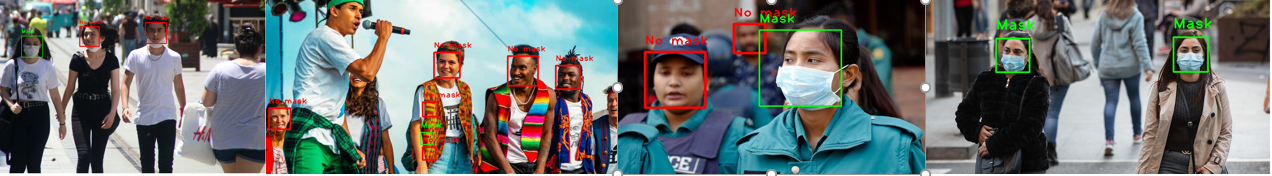
\includegraphics[width=1\textwidth]{test_image.PNG}
\centering
\caption{Some randomly chosen test results from unseen images.}
\label{testresult}
\end{figure}

\subsection{Discussion}

In this work, using deep learning model we proposed a novel application that is capable of distinguishing masked and non-masked human faces from videos and still pictures. Our experimental results proved that with a few limitations, with $98\%$ of accuracy our work is performing better than other related works reported when trained and tested on all image sets while in some cases a few of the comparative studies are performing better when focused on smaller and concentrated data set. 

\section{Limitations and Future Works}

One of this work's limitations is that for profile face images/videos, the proposed method is not working well, because of lack of the training images of profile faces. We have not tested our system on blurry/noisy data as well. \\

\par We are in the process of collecting more profile faces and maks/no-mask images for images containing multiple faces. We area also adding simulated Additive White Gaussian Noise (AWGN) to our existing test images to experiment if it still producing similar range of accuracy. Also, for face  detection, instead of using Haar-Cascade face detection from OpenCV, our plan is to try YOLO-V5 or so to make the face detection easier and robust.
%
% ---- Bibliography ----
%
\begin{thebibliography}{10}
%
\bibitem {ge2017detecting}
Ge, S., Li, J., Ye, Q. and Luo, Z., 2017. Detecting masked faces in the wild with lle-cnns. In Proceedings of the IEEE Conference on Computer Vision and Pattern Recognition (pp. 2682-2690).

\bibitem {loey2020fighting}
Loey, M., Manogaran, G., Taha, M.H.N. and Khalifa, N.E.M., 2020. Fighting against COVID-19: A novel deep learning model based on YOLO-v2 with ResNet-50 for medical face mask detection. Sustainable Cities and Society, p.102600.

\bibitem {loey2020hybrid}
Loey, M., Manogaran, G., Taha, M.H.N. and Khalifa, N.E.M., 2020. A hybrid deep transfer learning model with machine learning methods for face mask detection in the era of the COVID-19 pandemic. Measurement, 167, p.108288.

\bibitem {mohan2020tiny}
Mohan, P., Paul, A.J. and Chirania, A., 2020. A Tiny CNN Architecture for Medical Face Mask Detection for Resource-Constrained Endpoints. arXiv preprint arXiv:2011.14858.

\bibitem {chen2020efficient}
Chen, S., Liu, W. and Zhang, G., 2020. Efficient Transfer Learning Combined Skip-Connected Structure for Masked Face Poses Classification. IEEE Access, 8, pp.209688-209698.

\bibitem {chowdary2020face}
Chowdary, G.J., Punn, N.S., Sonbhadra, S.K. and Agarwal, S., 2020. Face Mask Detection using Transfer Learning of InceptionV3. arXiv preprint arXiv:2009.08369.

\bibitem {ourVideo}
A Test Video by the Authors. \url{https://youtu.be/1uLkBke2dGo}

\bibitem {kagglefacemask}
Face Mask Detection data set by Kaggle. \url{https://www.kaggle.com/andrewmvd/face-mask-detection}

\bibitem {smfd}
Simulated Masked Face Dataset (SMFD). \url{https://github.com/prajnasb/observations/tree/master/experiements}

\bibitem {wang2020masked}
Wang, Z., Wang, G., Huang, B., Xiong, Z., Hong, Q., Wu, H., Yi, P., Jiang, K., Wang, N., Pei, Y. and Chen, H., 2020. Masked face recognition dataset and application. arXiv preprint arXiv:2003.09093.

\bibitem {chandrikadeb7}
 Face-Mask-Detection Dataset. \url{https://github.com/chandrikadeb7/Face-Mask-Detection}

\bibitem {realAndFakeFace}
Real and Fake Face Detection. \url{https://www.kaggle.com/ciplab/real-and-fake-face-detection}

\bibitem {learned2016labeled}
Cabani, A., Hammoudi, K., Benhabiles, H. and Melkemi, M., 2020. MaskedFace-Net–A dataset of correctly/incorrectly masked face images in the context of COVID-19. Smart Health, p.100144.

\end{thebibliography}
\end{document}
